% --------------------------------------------------------------
% This is all preamble stuff that you don't have to worry about.
% Head down to where it says "Start here"
% --------------------------------------------------------------
 
\documentclass[12pt]{article}
 
\usepackage[margin=1in]{geometry} 
\usepackage{bm} % bold in mathmode \bm
\usepackage{amsmath,amsthm,amssymb,mathtools}
\usepackage{dsfont} % for indicator function \mathds 1
\usepackage{tikz,pgf,pgfplots}
\usepackage{enumerate} 
\usepackage[multiple]{footmisc} % for an adjascent footnote
\usepackage{graphicx,float} % figures

\newtheorem{definition}{Definition}
\let\olddefinition\definition
\renewcommand{\definition}{\olddefinition\normalfont}
\newtheorem{lemma}{Lemma}
\let\oldlemma\lemma
\renewcommand{\lemma}{\oldlemma\normalfont}
\newtheorem{proposition}{Proposition}
\let\oldproposition\proposition
\renewcommand{\proposition}{\oldproposition\normalfont}
\newtheorem{corollary}{Corollary}
\let\oldcorollary\corollary
\renewcommand{\corollary}{\oldcorollary\normalfont}
\newtheorem{theorem}{Theorem}
\let\oldtheorem\theorem
\renewcommand{\theorem}{\oldtheorem\normalfont}

\newcommand\norm[1]{\left\lVert#1\right\rVert} % \norm command 

%%% PLOTTING PARAMETERS
\tikzstyle{bag} = [text width=7em, text centered] %binomial tree node width
\tikzstyle{end} = []
%%%

%% set noindent by default and define indent to be the standard indent length
\newlength\tindent
\setlength{\tindent}{\parindent}
\setlength{\parindent}{0pt}
\renewcommand{\indent}{\hspace*{\tindent}}

\newcommand*{\vv}[1]{\vec{\mkern0mu#1}} % \vec command

%% DAVIDS MACRO KIT %%
\newcommand{\R}{\mathbb R}
\newcommand{\N}{\mathbb N}
\newcommand{\Z}{\mathbb Z}
\renewcommand{\P}{\mathbb P}
\newcommand{\Q}{\mathbb Q}
\newcommand{\E}{\mathbb E}
\newcommand{\var}{\mathrm{Var}}
\newcommand{\indist}{\,{\buildrel \mathcal D \over \sim}\,}

\newcommand{\bigtau}{\text{{\large $\bm \tau$}}}

\begin{document}
 
% --------------------------------------------------------------
%                         Start here
% --------------------------------------------------------------
 
\title{Assignment 2}
\author{David Fleischer -- 27101449\\ 
MACF 401 - Mathematical \& Computational Finance I}
\date{Due: February 4 2016 \\ Last update: \today{}}
\maketitle

\section*{Part I}

{\bf Solution 2.4.i:} We see that $M_0 = 0$ is constant and so it is measurable/adapted. For $n \geq 1$ we have $M_n$ depending only on the first $n$ coin tosses by its construction. Therefore we have that $M_n$ is adapted, satisfying the first condition. \\

Now, checking the martingale property of $M_n$:
\begin{align*}
	\E_n[M_{n + 1}] &= \E_n \left[ \sum^{n + 1}_{j = 1} X_j \right] \\
	&= \E_n \left[ \sum^{n}_{j = 1} X_j + X_{n + 1} \right] \\ 
	&= \E_n \left[ \sum^n_{j = 1} X_j \right] + \E_n \left[ X_{n + 1} \right] \quad \text{(by linearity)} \\
	&= \E_n [M_n] + \E_n \left[ X_{n + 1} \right] \quad \text{(by definition of $M_n$)} \\
	&= M_n + \E_n \left[ X_{n + 1} \right] \quad  \text{(since $M_n$ is known at the $n$th toss)} \\
	&= M_n + \E [X_{n + 1}] \quad \text{(since $X_{n + 1}$ is independent of the first $n$ tosses)} \\
	&= M_n + [ p\cdot(1) + q\cdot(-1) ] \quad \text{(by definition of ordinary expectation)} \\
	&= M_n + \left[ \frac{1}{2} - \frac{1}{2} \right] \\
	&= M_n
\end{align*}

\indent Therefore, since $M_n$ is both adapted and satisfies the martingale property we have that $M_n$ is a martingale, as desired. \\

{\bf Solution 2.4.ii:} We have that $S_n$ is a function of an adapted process 
\begin{equation*}
	f(S_n) = S_n = e^{\sigma M_n} \left( \frac{2}{e^{\sigma} + e^{-\sigma}} \right) ^n
\end{equation*}

\indent By the construction of $S_n$ it does not introduce dependency on any coin tosses beyond $n$ (in fact, $f$ does not introduce any further dependency on any coin toss beyond those used in $M_n$). Hence, $S_n$ depends only on the first $n$ coin tosses. Therefore we have that $S_n$ is adapted. \\

Confirming the martingale property of $S_n$:
\begin{align*}
	\E_n \left[ S_{n + 1} \right] &= \E_n \left[ e^{\sigma M_{n + 1}} \left( \frac{2}{e^{\sigma} + e^{-\sigma}} \right)^{n + 1} \right] \\
	&= \E_n \left[ e^{\sigma (M_n + X_{n + 1})} \left( \frac{2}{e^{\sigma} + e^{-\sigma}} \right)^{n + 1} \right] \quad \text{(from part (i))} \\
	&= \E_n \left[ e^{\sigma M_n} e^{\sigma X_{n + 1}} \left( \frac{2}{e^{\sigma} + e^{-\sigma}} \right)^{n + 1} \right] \\
	&= e^{\sigma M_n}\left( \frac{2}{e^{\sigma} + e^{-\sigma}} \right)^{n + 1} \E_n \left[ e^{\sigma X_{n + 1}} \right]  \quad \text{(taking out what is known)} \\
	&= e^{\sigma M_n}\left( \frac{2}{e^{\sigma} + e^{-\sigma}} \right)^n \E \left[ e^{\sigma X_{n + 1}} \right]  \quad \text{(since $X_{n + 1}$ is independent of the first $n$ tosses)} \\
	&= e^{\sigma M_n}\left( \frac{2}{e^{\sigma} + e^{-\sigma}} \right)^{n + 1} \left[ p\cdot e^{\sigma\cdot(1)} + q\cdot e^{\sigma\cdot(-1)} \right] \\
	&= e^{\sigma M_n}\left( \frac{2}{e^{\sigma} + e^{-\sigma}} \right)^{n + 1} \left[ \frac{1}{2}e^{\sigma} + \frac{1}{2} e^{-\sigma} \right] \\
	&= e^{\sigma M_n}\left( \frac{2}{e^{\sigma} + e^{-\sigma}} \right)^{n + 1} \frac{ e^{\sigma} + e^{-\sigma} }{2} \\
	&= e^{\sigma M_n}\left( \frac{2}{e^{\sigma} + e^{-\sigma}} \right)^n \\
	&= S_n
\end{align*}

\indent Therefore, since $S_n$ is both adapted and satisfies the martingale property we have that $S_n$ is a martingale, as desired. \\

{\bf Solution 2.5.i:} We reasons which will become clear through the solution, instead consider $2I_n$. We will show that $2I_n = M_n^2 - n$. So,
\begin{align*}
		2I_n &= 2\sum^{n - 1}_{j = 0} M_j(M_{j + 1} - M_j) \quad \text{(by definition)} \\
		&= 2 \sum^{n - 1}_{j = 0} \left( M_jM_{j + 1} - M_j^2 \right) \\
		&= 2\sum^{n - 1}_{j = 0} M_jM_{j + 1} - 2\sum^{n - 1}_{j = 0} M_j^2 
\end{align*}

but
\begin{align*}
	M_n^2 &= \sum^{n - 1}_{j = 0} M_{j + 1}^2 - \sum^{n - 1}_{j = 0} M_j^2 \\
	\implies \sum^{n - 1}_{j = 0} M_j^2 &= \sum^{n - 1}_{j = 0} M_{j + 1}^2 - M_n^2
\end{align*}

so
\begin{align*}
	2I_n &= 2\sum^{n - 1}_{j = 0} M_jM_{j + 1} - 2\sum^{n - 1}_{j = 0} M_j^2  \\
	&= 2\sum^{n - 1}_{j = 0} M_jM_{j + 1} - \sum^{n - 1}_{j = 0}M_j^2 - \left( \sum^{n - 1}_{j = 0} M_{j + 1}^2 - M_n^2 \right) \\
	&= 2\sum^{n - 1}_{j = 0} M_jM_{j + 1} - \sum^{n - 1}_{j = 0}M_j^2 - \sum^{n - 1}_{j = 0} M_{j + 1}^2 + M_n^2 \\
	&= M_n^2 + \sum^{n - 1}_{j = 0} \left( 2M_jM_{j + 1} - M_j^2 - M_{j + 1}^2 \right) \\
	&= M_n^2 - \sum^{n - 1}_{j = 0} \left(M_{j + 1} - M_j \right)^2 \\
	&= M_n^2 - \sum^{n - 1}_{j = 0} X_{j + 1}^2 \\
	&= M_n^2 - \sum^{n - 1}_{j = 0} 1 \\
	&= M_n^2 - n
\end{align*}

Hence
\begin{align*}
	2I_n &= M_n^2 - n \\
	\implies I_n &= \frac{1}{2}M_n^2 - \frac{1}{2}n
\end{align*}

as desired. \\

{\bf Solution 2.5.ii:}

\begin{align*}
	\E_n \left[ f(I_{n + 1}) \right] &= \E_n \left[ f \left( \sum^n_{j = 0} M_j(M_{j + 1} - M_j) \right) \right] \quad \text{(by definition)} \\
	&= \E_n \left[ f \left( \sum^{n - 1}_{j = 0} M_j(M_{j + 1} - M_j) + M_n(M_{n + 1} - M_n) \right) \right] \\
	&= \E_n \left[ f(I_n + M_nX_{n + 1}) \right]
\end{align*}

\indent However, $I_n$ and $M_n$ are adapted to the first $n$ coin tosses and $X_{n + 1}$ is independent of the first $n$ tosses. Therefore, our conditional expectation may be rewritten as the ordinary expectation
\begin{align*}
 	\E_n \left[ f(I_{n + 1}) \right] &= \E_n \left[ f(I_n + M_nX_{n + 1}) \right] \\
 	&= \E \left[ f(I_n + M_nX_{n + 1}) \right] \quad \text{(by the Independence Lemma)} \\
 	&= p\cdot f(I_n + M_n\cdot(1)) + q\cdot f(I_n + M_n\cdot(-1)) \\
 	&= \frac{1}{2} f(I_n + M_n) + \frac{1}{2} f(I_n - M_n)
\end{align*}

but we're offended by the presence of $M_n$ in our solution, so, from part (i),
\begin{align*}
	I_n &= \frac{1}{2}M_n^2 - \frac{1}{2}n \\
	\implies M_n &= \sqrt{2I_n + n}
\end{align*}

Hence
\begin{align*}
 	\E_n \left[ f(I_{n + 1}) \right] &= \frac{1}{2} f(I_n + M_n) + \frac{1}{2} f(I_n - M_n) \\
 	&= \frac{1}{2} f(I_n + \sqrt{2I_n + n}) + \frac{1}{2} f(I_n - \sqrt{2I_n + n}) \\
\end{align*}

Therefore
\begin{equation*}
	\E_n[f(I_{n + 1})] = g(I_n)
\end{equation*}

where
\begin{equation*}
	g(i) = \frac{1}{2}f(i + \sqrt{2i + n}) + \frac{1}{2}f(i - \sqrt{2i + n})
\end{equation*}

as desired. \\

{\bf Solution 2.8.i}: From the ``multistep-ahead'' version of the martingale property (equation 2.4.3) we have, for $0 \leq n \leq m \leq N$,
\begin{equation*}
	M_n = \E_n [M_m]
\end{equation*}

So, since $M_n$ and $M_n'$ are martingales, with $m = n$, for $0 \leq n \leq N$
\begin{align*}
	\tilde{\E}_n[M_N] &= M_n \\
	\tilde{\E}_n[M_N'] &= M_n'
\end{align*}

Hence, if $M_N = M_N'$
\begin{align*}
	\tilde{\E}_n[M_N] &= \tilde{\E}_n[M_N'] \\
	\implies M_n &= M_n'
\end{align*}

for arbitrary $0 \leq n \leq N$, as desired. \\

{\bf Solution 2.8.ii:} Let $V_N$ be the time $N$ payoff of a derivative security. Define the process $\{V_n\}^N_{n = 0}$ to be the derivative security price process such that
\begin{equation*}
	V_n(\omega_1\cdots\omega_n) = \frac{1}{1 + r} \left[ \tilde{p}V_{n + 1}(\omega_1\cdots\omega_n H) + \tilde{q}V_{n + 1}(\omega_1\cdots\omega_n T) \right] \quad \star
\end{equation*}

\indent By the construction of $V_n$ from equation (1.2.16) we see that $V_n$ is only dependent on the first $n$ coin tosses $(\omega_1\cdots\omega_n)$, hence $V_n$ is adapted. Now, confirming the martingale property
\begin{align*}
	\tilde{\E}_n \left[ \frac{V_{n + 1}}{(1 + r)^{n + 1}} \right] &= \frac{1}{(1 + r)^{n + 1}} \tilde{\E}_n \left[ V_{n + 1} \right] \quad \text{(taking out what is known)} \\
	&= \frac{1}{(1 + r)^{n + 1}} \left[ \tilde{p}V(H) + \tilde{q}V(T) \right] \\
	&= \frac{1}{(1 + r)^{n + 1}}(1 + r)V_n \quad \text{(from $\star$)} \\
	&= \frac{V_n}{(1 + r)^n}
\end{align*}

Hence
\begin{equation*}
	V_0, \frac{V_1}{1 + r}, \cdots, \frac{V_{N - 1}}{(1 + r)^{N - 1}}, \frac{V_N}{(1 + r)^N}
\end{equation*}
is a martingale under $\tilde{\P}$, as desired. \\

{\bf Solution 2.8.iii:} Once again, by the same argument as in (ii), we see that $V'_n$ depends only on the first $n$ tosses. That is, $V'_n$ is adapted. Now, for $0 \leq n \leq m \leq N$,
\begin{align*}
	\tilde{\E}_n \left[ \frac{V_{n + 1}}{(1 + r)^{n + 1}} \right] &= \tilde{\E}_n \left[  \frac{1}{(1 + r)^{n + 1}} \tilde{\E}_{n + 1} \left[ \frac{V_N}{(1 + r)^{N - (n + 1)}} \right] \right] \\
	&= \frac{1}{(1 + r)^n} \tilde{\E}_n \left[ \tilde{\E}_{n + 1} \left[ \frac{V_N}{(1 + r)^{N - n}} \right] \right] \quad \text{(taking out what is known)} \\
	&= \frac{1}{(1 + r)^n} \tilde{\E}_n \left[ \frac{V_N}{(1 + r)^{N - n}} \right] \quad \text{(by the tower property)} \\
	&= \frac{V'_n}{(1 + r)^n} \quad \text{(by definition)}
\end{align*}

Hence
\begin{equation*}
	V'_0, \frac{V'_1}{1 + r)}, \cdots, \frac{V'_{N - 1}}{(1 + r)^{N - 1}}, \frac{V_N}{(1 + r)^N}
\end{equation*}

is a martingale under $\tilde{\P}$, as desired. \\

{\bf Solution 2.8.iv:} We have from parts (ii) and (iii) that
\begin{align*}
\begin{cases}
	V_0, \frac{V_1}{1 + r}, \cdots, \frac{V_{N - 1}}{(1 + r)^{N - 1}}, \frac{V_N}{(1 + r)^N} \\
	V'_0, \frac{V'_1}{1 + r)}, \cdots, \frac{V'_{N - 1}}{(1 + r)^{N - 1}}, \frac{V_N}{(1 + r)^N}
\end{cases}
\end{align*}

are martingales under $\tilde{\P}$. Additionally, we have that at time $N$ both processes have the same terminal value $V_N$. Therefore, by part (i) we must have that $V_n = V'_n$ for arbitrary $0 \leq n \leq N$, as desired. \\

{\bf Solution 2.9.i:} We first compute the up \& down factors at each node
\begin{align*}
	u_0 &= \frac{S_1(H)}{S_0} = \frac{8}{4} = 2 \\
	d_0 &= \frac{S_1(T)}{S_0} = \frac{2}{4} = \frac{1}{2} \\
	u_1(H) &= \frac{S_2(HH)}{S_1(H)} = \frac{12}{8} = \frac{3}{2} \\
	d_1(H) &= \frac{S_2(HT)}{S_1(H)} = \frac{8}{8} = 1 \\
	u_1(T) &= \frac{S_2(TH)}{S_1(T)} = \frac{8}{2} = 4 \\
	d_1(T) &= \frac{S_2(TT)}{S_1(T)} = \frac{2}{2} = 1
\end{align*}

Thus, 
\begin{align*}
	\tilde{p}_0 &= \frac{(1 + r_0) - d_0}{u_0 - d_0} = \frac{(1 + \frac{1}{4}) - \frac{1}{2}}{2 - \frac{1}{2}} = \frac{ \frac{3}{4} }{ \frac{3}{2} } = \frac{6}{12} = \frac{1}{2} \\
	\implies \tilde{q}_0 &= 1 - \tilde{p}_0 = \frac{1}{2} \\
	\tilde{p}_1(H) &= \frac{(1 + r_1(H)) - d_1(H)}{u_1(H) - d_1(H)} = \frac{1 + \frac{1}{4} - 1}{\frac{3}{2} - 1} = \frac{ \frac{1}{4} }{ \frac{1}{2} } = \frac{1}{2} \\
	\implies \tilde{q}_1(H) &= 1 - \tilde{p}_1(H) = \frac{1}{2} \\
	\tilde{p}_1(T) &= \frac{(1 + r_1(T)) - d_1(T)}{u_1(T) - d_1(T)} = \frac{1 + \frac{1}{2} - 1}{4 - 1} = \frac{ \frac{1}{2} }{3} = \frac{1}{6} \\
	\implies \tilde{q}_1(T) &= 1 - \tilde{p}_1(T) = \frac{5}{6}
\end{align*}

Therefore, by the independence of the coin tosses,
\begin{align*}
	\tilde{\P}(HH) &= \tilde{p}_0\tilde{p}_1(H) = \frac{1}{2}\cdot\frac{1}{2} = \frac{1}{4} \\
	\tilde{\P}(HT) &= \tilde{p}_0\tilde{q}_1(H) = \frac{1}{2}\cdot\frac{1}{2} = \frac{1}{4} \\
	\tilde{\P}(TH) &= \tilde{q}_0\tilde{p}_1(T) = \frac{1}{2}\cdot\frac{1}{6} = \frac{1}{12} \\
	\tilde{\P}(TT) &= \tilde{q}_0\tilde{p}_1(T) = \frac{1}{2}\cdot\frac{5}{6} = \frac{5}{12} \\
\end{align*}

as desired. \\

{\bf Solution 2.9.ii:} Going backwards through our tree
\begin{align*}
	V_1(H) &= \frac{1}{1 + r_1(H)}[\tilde{p}_1(H)V_2(HH) + \tilde{q}_1(H)V_2(HT)] \\
	&= \frac{4}{5}\left[ \frac{1}{2}\cdot 5 + \frac{1}{2}\cdot 1 \right] \\
	&= \frac{12}{5} = 2.4 \\
	V_1(T) &= \frac{1}{1 + r_1(T)}[\tilde{p}_1(T)V_2(TH) + \tilde{q}_1(T)V_2(TT)] \\
	&= \frac{2}{3} \left[ \frac{1}{6} \cdot 1 + \frac{5}{6} \cdot 0 \right] \\
	&= \frac{1}{9} = 0.111...
\end{align*}

Hence
\begin{align*}
	V_0 &= \frac{1}{1 + r_0}[\tilde{p}_0V_1(H) + \tilde{q}_0V_1(T)] \\
	&= \frac{4}{5} \left[ \frac{1}{2} \cdot \frac{12}{5} + \frac{1}{2} \cdot \frac{1}{9} \right] \\
	&= \frac{226}{225} = 1.00444...
\end{align*}

{\bf Solution 2.9.iii:} Recalling our formula for $\Delta_0$ we have
\begin{align*}
	\Delta_0 &= \frac{ V_1(H) - V_1(T) }{ S_1(H) - S_1(T) } \\
	&= \frac{ \frac{12}{5} - \frac{1}{9} }{ 8 - 2 } \\
	&= \frac{103}{270} = 0.3\overline{814}
\end{align*}

{\bf Solution 2.9.iv:} Once again
\begin{align*}
	\Delta_1 &= \frac{ V_1(HH) - V_1(HT) }{ S_1(HH) - S_1(HT) } \\
	&= \frac{ 5 - 1 }{ 12 - 8 } \\
	&= 1
\end{align*}

\section*{Part II}

{\bf Solution 1.a:} We first note that $J_k(\omega_1\cdots\omega_k)$ is a function of the first $k$ coin tosses, namely, the value $J_k$ takes will depend on the $k$th coin toss. Hence, $J_k$ is adapted since it does not rely on information beyond time $k$. Now, we have that $Y_k$ is a function of deterministic variables $k, p$ and random variables $J_i$. We have already determined that $J_i$ is adapted and so, since $Y_k$ introduces no further dependency on any coin tosses, we may state that $Y_k$ is in fact adapted. \\

Now, to confirm that the martingale property holds
\begin{align*}
	\E_k \left[ Y_{k + 1} \right] &= \E_k \left[ \sum^{k + 1} _{i = 0} J_i - (k + 1)p \right] \quad \text{(by definition)} \\
	&= \E_k \left[ \sum^k_{i = 0} J_i + J_{k + 1} - kp - p \right] \\
	&= \E_k \left[ Y_k + J_{k + 1} - p \right] \\
	&= \E_k \left[ Y_k - p \right] + \E_k \left[ J_{k + 1} \right] \quad \text{(linearity)} \\
	&= Y_k - p + \E_k \left[ J_{k + 1} \right] \quad \text{(since $Y_k$ and $p$ are known at $k$)}
\end{align*}

but we have that $J_{k + 1}$ is independent of the first $k$ coin tosses since its value is uniquely determined by the $(k + 1)$th coin toss, hence
\begin{align*}
	\E_k \left[ Y_{k + 1} \right] &= Y_k - p + \E_k \left[ J_{k + 1} \right] \\
	&= Y_k - p + p\cdot(1) + (1 - p)\cdot(0) \\
	&= Y_k - p + p \\
	&= Y_k
\end{align*}

\indent Therefore, since $Y_k$ is adapted and satisfies the martingale property we may conclude that $Y_k$ is in fact a martingale, as desired. \\


{\bf Solution 1.b:} From part (a) we have that $Y_k$ is adapted. Now, to confirm that the Markov property holds
\begin{align*}
	\E_k \left[ f(Y_{k + 1}) \right] &= \E_k \left[ f \left( \sum^{k + 1}_{i = 1} J_i - (k + 1)p \right) \right] \\ 
	&= \E_k \left[ f \left( \sum^k_{i = 1} J_i + J_{k + 1} - kp - p \right) \right] \\
	&= \E_k \left[ f \left( Y_k - J_{k + 1} - p \right) \right]
\end{align*}

\indent We now note that $Y_k$ is adapted to the first $k$ coin tosses, $p$ some constant $0 < p < 1$, and $J_{k + 1}$ is independent of the first $k$ coin tosses. That is, we have that $Y_k$ and $p$ is measurable with respect to the information up to $k$ and $J_{k + 1}$ is independent of this information, therefore, by the Independence Lemma we have that
\begin{equation*}
	\E_k \left[ f \left( Y_k - J_{k + 1} - p \right) \right] = g(Y_k)
\end{equation*}

such that $g$ is the ordinary expectation
\begin{align*}
	g(y) &= \E \left[ f \left( y - J_{k + 1} - p \right) \right] \\
	&= p \cdot f(y + (1) - p) + (1 - p) \cdot f(y + (0) - p) \\
	&= pf(y + 1 - p) + (1 - p)f(y - p)
\end{align*}

\indent Since we have that $Y_k$ is adapted and have successfully found a function $g$ for arbitrary $f$ such that
\begin{equation*}
	\E_k \left[ f(Y_{k + 1}) \right] = g(Y_k)
\end{equation*}

we may conclude that the process $\{Y_k\}^N_{k = 0}$ is Markovian, as desired. \\

{\bf Solution 2.a:} We first consider the asset price tree. Since the option value is clearly path dependent we construct the following non-recombining tree for later use in determining the derivative price
\begin{figure}[H]
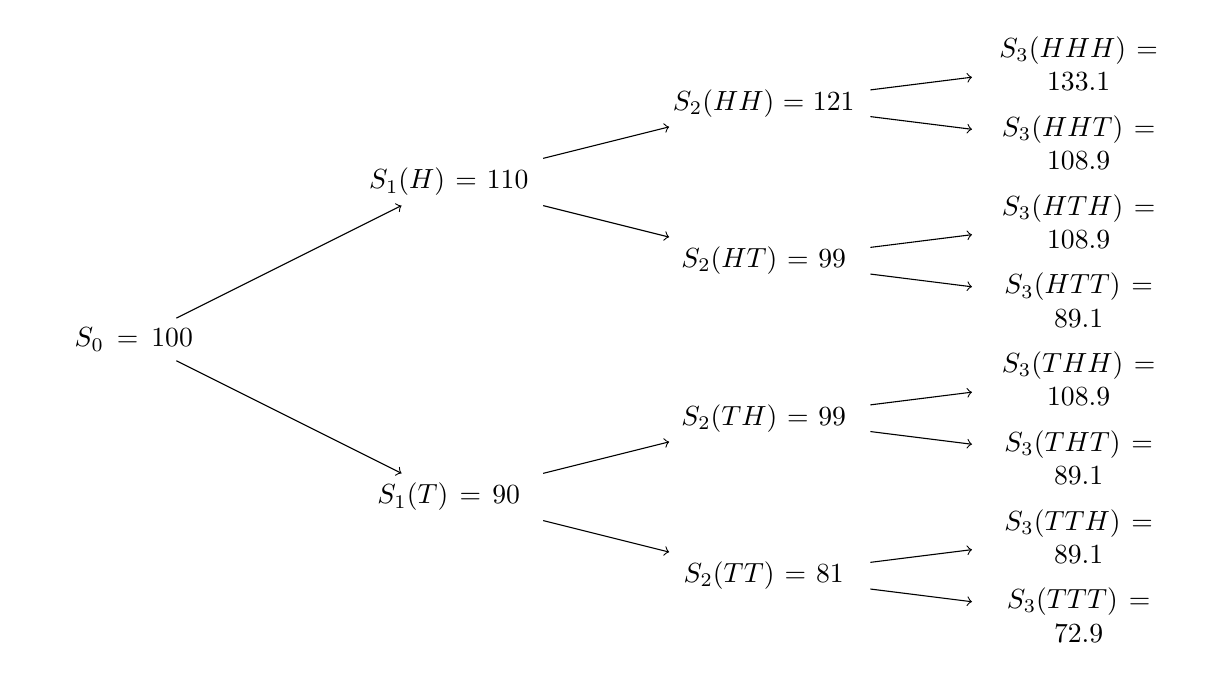
\begin{tikzpicture}[sloped]
  \node (a) at ( 0,0) [bag] {$S_0 = 100$};
  \node (b) at ( 4,-2) [bag] {$S_1(T) = 90$};
  \node (c) at ( 4,2) [bag] {$S_1(H) = 110$};
  \node (d) at ( 8,-3) [bag] {$S_2(TT) = 81$};
  \node (e) at ( 8,-1) [bag] {$S_2(TH) = 99$};
  \node (f) at ( 8,1) [bag] {$S_2(HT) = 99$};
  \node (g) at ( 8,3) [bag] {$S_2(HH) = 121$};
  \node (h) at ( 12,-3.5) [bag] {$S_3(TTT) = 72.9$};
  \node (i) at ( 12,-2.5) [bag] {$S_3(TTH) = 89.1$};
  \node (j) at ( 12,-1.5) [bag] {$S_3(THT) = 89.1$};
  \node (k) at ( 12,-0.5) [bag] {$S_3(THH) = 108.9$};
  \node (l) at ( 12,0.5) [bag] {$S_3(HTT) = 89.1$};
  \node (m) at ( 12,1.5) [bag] {$S_3(HTH) = 108.9$};
  \node (n) at ( 12,2.5) [bag] {$S_3(HHT) = 108.9$};
  \node (o) at ( 12,3.5) [bag] {$S_3(HHH) = 133.1$};
  \draw [->] (a) to node [below] {} (b);
  \draw [->] (a) to node [above] {} (c);
  \draw [->] (b) to node [below] {} (d);
  \draw [->] (b) to node [above] {} (e);
  \draw [->] (c) to node [below] {} (f);
  \draw [->] (c) to node [above] {} (g);
  \draw [->] (d) to node [below] {} (h);
  \draw [->] (d) to node [above] {} (i);
  \draw [->] (e) to node [below] {} (j);
  \draw [->] (e) to node [above] {} (k);
  \draw [->] (f) to node [below] {} (l);
  \draw [->] (f) to node [above] {} (m);
  \draw [->] (g) to node [above] {} (n);  
  \draw [->] (g) to node [above] {} (o);  
\end{tikzpicture}
\caption{Asset price process tree}
\end{figure}

Now, at time 3 we have the option payoff
\begin{equation*}
	V_3(\omega_1\omega_2\omega_3) = (S_3(\omega_1\omega_2\omega_3) - K)^+ \cdot \prod^3_{i = 1} \mathds 1_{ \{ S_i(\omega_1\cdots\omega_i) > B \} }
\end{equation*}

So, with strike $K = 105$ and barrier $B = 95$
\begin{align*}
	V_3(HHH) &= (133.1 - 105)^+ \cdot 1 = 28.1 \\
	V_3(HHT) &= (108.9 - 105)^+ \cdot 1 = 3.9 \\
	V_3(HTH) &= (108.9 - 105)^+ \cdot 1 = 3.9 \\
	V_3(HTT) &= (89.1 - 105)^+ \cdot 0 = 0 \\
	V_3(THH) &= (108.9 - 105)^+ \cdot 0 = 0\\
	V_3(THT) &= (89.1 - 105)^+ \cdot 0 = 0 \\
	V_3(TTH) &= (89.1 - 105)^+ \cdot 0 = 0 \\
	V_3(TTT) &= (72.9 - 105)^+ \cdot 0 = 0
\end{align*}

and determining the risk-neutral probabilities
\begin{align*}
	\tilde{p} &= \frac{(1 + r) - d}{u - d} = \frac{(1 + (e^{0.05} - 1)) - 0.9}{1.1 - 0.9} = \frac{e^{0.05} - 0.9}{0.2} = 5e^{0.05} - 4.5 \approx 0.7563\,5548 \\
	\implies \tilde{q} &= 1 - \tilde{p} = 1 - (5e^{0.05} - 4.5) = 5.5 - 5e^{0.05} \approx 0.2346\,4451
\end{align*}

\indent From these values it is quick work to fill in the remaining nodes of the non-recombining derivative price tree
\begin{align*}
	V_2(HH) &= \frac{1}{1 + r} [\tilde{p}V_3(HHH) + \tilde{q}V_3(HHT)] \\
	&= \frac{1}{1 + (e^{0.05} - 1)} [0.7563\,5548 \cdot (28.1) + 0.2346\,4451 \cdot (3.9)] \\
	&= e^{-0.05} \cdot 22.1687\,0257 \\
	&= 21.0875\,2219 \\
	V_2(HT) &= \frac{1}{1 + r} [\tilde{p}V_3(HTH) + \tilde{q}V_3(HTT)] \\
	&= \frac{1}{1 + (e^{0.05} - 1)} [0.7563\,5548 \cdot (3.9) + 0.2346\,4451 \cdot (0) ]  \\
	&= e^{-0.05} \cdot 2.9497\,8637 \\
	&= 2.8059\,2359 \\
	V_2(TH) &= \frac{1}{1 + r} [\tilde{p}V_3(THH) + \tilde{q}V_3(THT)] \\
	&= \frac{1}{1 + (e^{0.05} - 1)} [0.7563\,5548 \cdot (0) + 0.2346\,4451 \cdot (0) ] \\
	&= e^{-0.05} \cdot 0 \\
	&= 0 \\
	V_2(TT) &= \frac{1}{1 + r} [\tilde{p}V_3(TTH) + \tilde{q}V_3(TTT)] \\
	&= \frac{1}{1 + (e^{0.05} - 1)} [0.7563\,5547 (0) \cdot + 0.2346\,4451 \cdot (0)] \\
	&= e^{-0.05} \cdot 0 \\
	&= 0
\end{align*}

and
\begin{align*}
	V_1(H) &= \frac{1}{1 + r}[\tilde{p}V_2(HH) + \tilde{q}V_2(HT)] \\
	&= \frac{1}{1 + (e^{0.05} - 1)} [0.7563\,5547 \cdot (21.0875\,2219) + 0.2346\,4451 \cdot (2.8059\,2359) ] \\
	&= e^{-0.05} \cdot 16.6080\,5753 \\
	&= 15.7980\,7301 \\
	V_1(T) &= \frac{1}{1 + r}[\tilde{p}V_2(TH) + \tilde{q}V_2(TT)] \\
	&= \frac{1}{1 + (e^{0.05} - 1)} [0.7563\,5547 \cdot 0 + 0.2346\,4451 \cdot 0] \\
	&= e^{-0.05} \cdot 0 \\
	&= 0
\end{align*}

Thus
\begin{align*}
	V_0 &= \frac{1}{1 + r}[ \tilde{p} V_1(H) + \tilde{q}V_1(T)] \\
	&= \frac{1}{1 + (e^{0.05} - 1)} [0.7563\,5547 \cdot (15.7980\,7301) + 0.2346\,4451 \cdot (0)] \\
	&= e^{-0.05} \cdot 11.9489\,5909 \\
	&= 11.3662\,0148
\end{align*}

as desired. \\

{\bf Solution 2.b:} We calculate our values for $\Delta_n$, $0 \leq n \leq 3$, at each node of the tree using
\begin{equation*}
	\Delta_n(\omega_1\cdots\omega_n) = \frac{ S_{n + 1}(\omega_1\cdots\omega_n H) - S_{n + 1}(\omega_1\cdots\omega_n T) }{ V_{n + 1}(\omega_1\cdots\omega_n H) - V_{n + 1}(\omega_1\cdots\omega_n T) }
\end{equation*}

Hence at time $t = 0$
\begin{align*}
	\Delta_0 &= \frac{V_1(H) - V_1(T)}{S_1(H) - S_1(T)} = \frac{15.7980\,7301 - 0}{110 - 90} = \frac{15.7980\,7301}{20} = 0.7899\,0365
\end{align*}

at time $t = 1$ we find
\begin{align*}
	\Delta_1(H) &= \frac{V_2(HH) - V_2(HT)}{S_2(HH) - S_2(HT)} = \frac{21.0875\,2219 - 2.8059\,2359}{121 - 99} = \frac{18.2815\,9860}{22} = 0.8309\,8175 \\
	\Delta_1(T) &= \frac{V_2(TH) - V_2(TT)}{S_2(TH) - S_2(TT)} = \frac{0 - 0}{99 - 81} = \frac{0}{18} = 0
\end{align*}

and finally at time $t = 2$
\begin{align*}
	\Delta_2(HH) &= \frac{V_3(HHH) - V_3(HHT)}{S_3(HHT) - S_3(HHT)} = \frac{28.1 - 3.9}{133.1 - 108.9} = \frac{24.2}{24.2} = 1 \\
	\Delta_2(HT) &= \frac{V_3(HTH) - V_3(HTT)}{S_3(HTH) - S_3(HTT)} = \frac{3.9 - 0}{108.9 - 89.1} = \frac{3.9}{19.8} = 0.1\overline{96} \\
	\Delta_2(TH) &= \frac{V_3(THH) - V_3(THT)}{S_3(THH) - S_3(THT)} = \frac{0 - 0}{108.9 - 89.1} = \frac{0}{19.8} = 0 \\
	\Delta_2(TT) &= \frac{V_3(TTH) - V_3(TTT)}{S_3(THH) - S_3(TTT)} = \frac{0 - 0}{89.1 - 72.9} = \frac{0}{16.2} = 0
\end{align*}

as desired.







































\end{document}
